\section{黏性解}
\label{sec:hj-viscosity}

折角处没有导数，方程不能代入。能否用一些有导数的东西替代它？答案是拿光滑函数从上方或下方贴住$u$，把方程写在贴住的光滑函数上。

\paragraph{用光滑函数从两侧接触}
设$\varphi$是光滑函数，$u-\varphi$在点$\bm{x}_0$有局部极大值。几何上，把$\varphi$上下平移，使它在$\bm{x}_0$处与$u$相等，那么附近有$\varphi\geq u$，$\varphi$从上方贴住$u$。若$u$在$\bm{x}_0$可微，极值点的一阶条件给出$\nabla\varphi(\bm{x}_0)=\nabla u(\bm{x}_0)$。这样可以从$\varphi$读出$u$的梯度。

$u$不可微时，情况由折角的方向决定。图~\ref{fig:hj-touching}画了三种情形。在光滑点上，从上方和下方都能贴住，贴住的函数斜率都等于$u$的斜率。在向下弯的折角（凹折角）处，从上方可以用多种斜率贴住，从下方则根本贴不住。在向上弯的折角（凸折角）处正好相反。

\begin{BookInlineFigure}
  \centering
  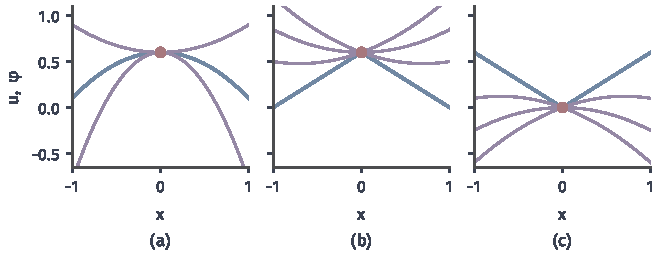
\includegraphics[width=112mm]{figures/06-differential-equations/02-partial-differential-equations/matplotlib/hj-touching/figure.pdf}
  \caption{光滑测试函数（紫）在红点贴住$u$（蓝）。(a)光滑点：上下两侧都能贴住，斜率唯一。(b)凹折角：只能从上方贴住，斜率可取一个区间。(c)凸折角：只能从下方贴住，斜率可取一个区间。}
  \label{fig:hj-touching}
\end{BookInlineFigure}

接下来决定不等式的方向。设$u_\varepsilon$是$\partial_tu+H(\nabla u)=\varepsilon\Delta u$的光滑解，$\varepsilon>0$，且$u_\varepsilon-\varphi$在内部点取局部极大。一阶条件和二阶条件给出
\[
  \partial_t\varphi=\partial_tu_\varepsilon,\qquad\nabla\varphi=\nabla u_\varepsilon,\qquad\Delta u_\varepsilon\leq\Delta\varphi.
\]
代入方程，得到
\[
  \partial_t\varphi+H(\nabla\varphi)=\varepsilon\Delta u_\varepsilon\leq\varepsilon\Delta\varphi.
\]
令$\varepsilon\to0$，右端趋于零。所以从上方贴时，自然的要求是$\partial_t\varphi+H(\nabla\varphi)\leq0$；从下方贴时不等号反向。这个计算只是启示，严格的结论在第~\ref{sec:hj-vanishing}节证明，但它已经给出了定义的形状。

\begin{definition}[黏性解]
\label{def:hj-viscosity}
设$u\in C(\mathbb{R}^{d}\times[0,t_{\mathrm{f}}))$。若对每个$\varphi\in C^1(\mathbb{R}^{d}\times(0,t_{\mathrm{f}}))$，当$u-\varphi$在$(\bm{x}_0,t_0)$（$t_0>0$）取局部极大值时都有
\begin{equation}
  \partial_t\varphi(\bm{x}_0,t_0)+H\bigl(t_0,\bm{x}_0,\nabla\varphi(\bm{x}_0,t_0)\bigr)\leq0,
  \label{eq:hj-subsolution}
\end{equation}
就称$u$是式~\eqref{eq:hj-ivp}中方程的\term{黏性次解}（viscosity subsolution）。若对每个这样的$\varphi$，当$u-\varphi$在$(\bm{x}_0,t_0)$取局部极小值时都有
\begin{equation}
  \partial_t\varphi(\bm{x}_0,t_0)+H\bigl(t_0,\bm{x}_0,\nabla\varphi(\bm{x}_0,t_0)\bigr)\geq0,
  \label{eq:hj-supersolution}
\end{equation}
就称$u$是\term{黏性上解}（viscosity supersolution）。既是次解又是上解的函数称为黏性解。初值问题的黏性解还要求$u(\cdot,0)=u_0$。
\end{definition}

记忆方式是：次解贴上方，得到“小于等于”；上解贴下方，得到“大于等于”。这个定义里从头到尾没有$u$的导数，所以它对连续函数有意义。

稳态方程$F(\bm{x},\nabla u)=0$的定义完全相同：局部极大处要求$F(\bm{x}_0,\nabla\varphi)\leq0$，局部极小处要求$F(\bm{x}_0,\nabla\varphi)\geq0$，边界条件单独提出。到达时间问题取
\[
  F(\bm{x},\bm{p})=c(\bm{x})\lVert\bm{p}\rVert_2-1.
\]

定义要有用，首先不能把经典解排除在外，而且不可微的地方之外应当和原方程一致。

\begin{lemma}[与经典解相容]
\label{lem:hj-consistency}
(1)连续可微的经典解是黏性解。(2)若黏性解$u$在内部点$\bm{z}_0=(\bm{x}_0,t_0)$可微，则方程在$\bm{z}_0$处逐点成立，即
\begin{equation}
  \partial_tu(\bm{z}_0)+H\bigl(t_0,\bm{x}_0,\nabla u(\bm{z}_0)\bigr)=0.
  \label{eq:hj-consistency}
\end{equation}
\end{lemma}

\begin{proof}
(1)若$u\in C^1$，$u-\varphi$在内部取极值，则$\partial_t\varphi=\partial_tu$，$\nabla\varphi=\nabla u$，代入方程得到等号，两个不等式都成立。

(2)只需构造一个$C^1$函数从上方贴住$u$且导数与$u$相同，下方同理，再分别代入两个定义。记$r=\lVert\bm{z}-\bm{z}_0\rVert_2$，并令$v$为$u$减去它在$\bm{z}_0$的一阶Taylor多项式。由可微性，
\[
  \rho(r)=\max_{\lVert\bm{z}-\bm{z}_0\rVert_2\leq r}\frac{\lvert v(\bm{z})\rvert}{\lVert\bm{z}-\bm{z}_0\rVert_2}
\]
连续、不减，且$\rho(0)=0$（规定分式在$\bm{z}=\bm{z}_0$处取$0$）。令
\[
  \psi(\bm{z})=\int_r^{2r}\rho(\tau)\,\mathrm{d}\tau.
\]

$\rho$连续，所以$\psi$在$\bm{z}\neq\bm{z}_0$处$C^1$。又$\lvert\psi\rvert\leq r\rho(2r)=o(r)$，所以$\psi$在$\bm{z}_0$处可微且导数为零，导数的表达式也趋于零，$\psi\in C^1$。由$\rho$不减，得$\psi(\bm{z})\geq r\rho(r)\geq v(\bm{z})$。

于是$v-\psi$在$\bm{z}_0$有局部极大值$0$，以“一阶Taylor多项式$+\psi$”作测试函数代入式~\eqref{eq:hj-subsolution}，得到式~\eqref{eq:hj-consistency}左端$\leq0$。用$-\psi$代替$\psi$，由式~\eqref{eq:hj-supersolution}得到$\geq0$。
\end{proof}

Lipschitz函数几乎处处可微（Rademacher定理，证明要用到Lebesgue微分定理和逐方向的论证，篇幅较长，读者可查阅实分析教材），所以Lipschitz连续的黏性解几乎处处满足方程。黏性解比“几乎处处解”多出来的，是在余下的零测集上的不等式。

下面的引理很快会用到：Lipschitz函数被贴住时，测试函数的斜率不会超过Lipschitz常数。

\begin{lemma}[贴住Lipschitz函数]
\label{lem:hj-lipschitz-touch}
设$u$关于$\bm{x}$是$R$-Lipschitz的，$\varphi\in C^1$，$u-\varphi$在$(\bm{x}_0,t_0)$取局部极大值或局部极小值，则
\begin{equation}
  \lVert\nabla\varphi(\bm{x}_0,t_0)\rVert_2\leq R.
  \label{eq:hj-lipschitz-touch}
\end{equation}
\end{lemma}

\begin{proof}
设取局部极大值，$t$固定为$t_0$。对单位向量$\bm{e}$和小$h>0$，有
\[
  \varphi(\bm{x}_0+h\bm{e},t_0)-\varphi(\bm{x}_0,t_0)\geq u(\bm{x}_0+h\bm{e},t_0)-u(\bm{x}_0,t_0)\geq-Rh.
\]
除以$h$并令$h\to0$，得到$\langle\nabla\varphi,\bm{e}\rangle\geq-R$。取$\bm{e}=-\nabla\varphi/\lVert\nabla\varphi\rVert_2$，就得到结论。局部极小的情形把$u-\varphi$换成$\varphi-u$。
\end{proof}

\paragraph{折角检验}
回到程函方程$\lvert u'\rvert=1$，$u(\pm1)=0$，这里$F(p)=\lvert p\rvert-1$。检验两个候选。

\begin{example}[两个折角]
\label{ex:hj-kink-test}
候选一$u=1-\lvert x\rvert$。在$x\neq0$处它光滑且满足方程，只需检验$x=0$。从下方贴不住（$x=0$是凹折角），所以上解条件是空的。从上方贴住时，$\varphi'(0)=p$满足$\lvert p\rvert\leq1$，于是
\[
  F(p)=\lvert p\rvert-1\leq0.
\]
次解条件成立，$1-\lvert x\rvert$是黏性解。

候选二$u=\lvert x\rvert-1$。$x=0$是凸折角，从上方贴不住，从下方能贴住。取$\varphi\equiv-1$，它从下方贴住$u$，斜率为$0$。上解条件要求
\[
  F(0)=-1\geq0,
\]
这不成立，所以$\lvert x\rvert-1$不是黏性解。
\end{example}

图~\ref{fig:hj-kink-test}展示了这两个检验。第~\ref{chap:pde-problems}章的每条锯齿线都有凸折角，同样在那里失败。凹折角和凸折角的差别就是答案：凸折角要求贴住的斜率长度至少为$1$，而$[-1,1]$内的斜率都能贴住，这不可能；凹折角要求长度至多为$1$，恰好成立。

\begin{BookInlineFigure}
  \centering
  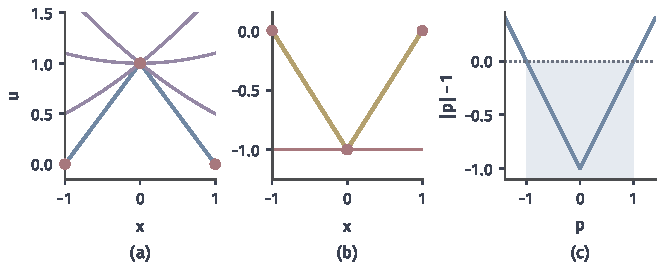
\includegraphics[width=112mm]{figures/06-differential-equations/02-partial-differential-equations/matplotlib/hj-kink-test/figure.pdf}
  \caption{程函方程$\lvert u'\rvert=1$（红点为边值）的折角检验。(a)$1-\lvert x\rvert$在顶点被紫线从上方贴住，斜率在$[-1,1]$内。(b)$\lvert x\rvert-1$在底点被水平红线从下方贴住，斜率$0$。(c)$\lvert p\rvert-1$，浅蓝范围内它不大于$0$：次解条件成立而上解条件不成立。}
  \label{fig:hj-kink-test}
\end{BookInlineFigure}

这个检验在到达时间问题中有直观的含义。若$T$在内部有凸折角，那么该点比它左右两边都早被到达，可是波前只能从相邻位置传来，内部没有源的地方不可能出现这种情况。凹折角则是两列波前相遇的地方，这是允许的。

定义对方程的符号敏感。把$F$换成$-F$，上下解的角色互换，方程$-\lvert u'\rvert+1=0$的黏性解是$\lvert x\rvert-1$，而不是$1-\lvert x\rvert$。这一点和弱解不同：弱形式乘$-1$不改变解集。这里的符号规定了信息传播的方向，$\partial_tu+H=0$中$\partial_tu$的系数为正，这是时间向前的方向。

对高维的到达时间问题，同样的两步检验可以直接做。

\begin{theorem}[距离函数]
\label{thm:hj-distance}
设$\Omega\subset\mathbb{R}^{d}$是开集，$\Omega\neq\mathbb{R}^{d}$，$u(\bm{x})$是$\bm{x}$到$\partial\Omega$的最短欧氏距离。则$u$是
\begin{equation}
  \lVert\nabla u\rVert_2-1=0\quad\text{在}\ \Omega\ \text{内}
  \label{eq:hj-distance}
\end{equation}
的黏性解。
\end{theorem}

\begin{proof}
三角不等式说明$u$是$1$-Lipschitz的。局部极大处，由引理~\ref{lem:hj-lipschitz-touch}得$\lVert\nabla\varphi\rVert_2\leq1$，次解条件成立。

设$u-\varphi$在$\bm{x}\in\Omega$取局部极小值，$\bm{y}\in\partial\Omega$是最近点，$\bm{e}$是从$\bm{x}$指向$\bm{y}$的单位向量。对小$h>0$，$\bm{x}_h=\bm{x}+h\bm{e}$仍在$\Omega$内，并且
\[
  u(\bm{x}_h)\leq\lVert\bm{x}_h-\bm{y}\rVert_2=u(\bm{x})-h.
\]
由局部极小，得到
\[
  \varphi(\bm{x}_h)-\varphi(\bm{x})\leq u(\bm{x}_h)-u(\bm{x})\leq-h.
\]
除以$h$并令$h\to0$，得到$\langle\nabla\varphi,\bm{e}\rangle\leq-1$，所以$\lVert\nabla\varphi(\bm{x})\rVert_2\geq1$，上解条件成立。
\end{proof}

取$\Omega=\mathbb{R}^2\setminus\{\bm{a},\bm{b}\}$，就知道图~\ref{fig:hj-two-sources}的$T=\min\{T_1,T_2\}$是黏性解。“第一次到达”这个物理选择，在方程层面就是黏性条件。

\paragraph{时间依赖的折角}
再回到凹槽$w$。它在$(0,t)$处的折角和$(t/2,t)$处的折角方向相反，检验结果也相反。

\begin{example}[凹槽不是黏性解]
\label{ex:hj-notch-test}
在$t_0>0$的点$(0,t_0)$附近，$w=\lvert x\rvert-t/2$。函数$\varphi=-t/2$从下方贴住$w$，其$q=\partial_t\varphi=-1/2$，$p=\partial_x\varphi=0$。上解条件要求
\[
  q+\frac{p^2}{2}=-\frac12\geq0,
\]
不成立，所以$w$不是上解。

对比$x=t/2$的折角。在那里$w=\min\{x-t/2,\ 0\}$，从上方贴住的测试函数，其$(q,p)$落在两个平面梯度$(-\tfrac12,1)$和$(0,0)$的连线上，写成$(q,p)=(-s/2,s)$，$0\leq s\leq1$。代入得到
\[
  q+\frac{p^2}{2}=-\frac{s}{2}+\frac{s^2}{2}\leq0,
\]
次解条件成立。这个折角是允许的。
\end{example}

图~\ref{fig:hj-notch-test}是这两个量。第一个折角对应$v$的左值小于右值的跳跃，第二个对应左值大于右值的跳跃，这和第~\ref{sec:hj-cusps}节由熵条件得到的判断一致。黏性解的定义不用导数，却自动区分了这两种跳跃。

\begin{BookInlineFigure}
  \centering
  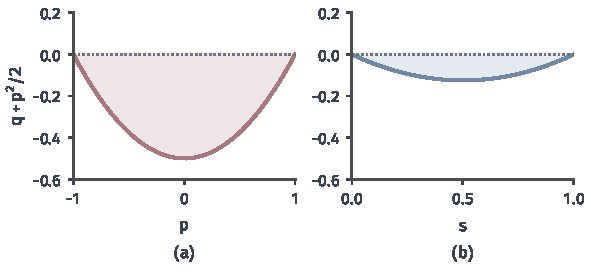
\includegraphics[width=100mm]{figures/06-differential-equations/02-partial-differential-equations/matplotlib/hj-notch-test/figure.pdf}
  \caption{凹槽$w$两类折角上的检验量$q+p^2/2$。(a)底部$x=0$处，$q=-1/2$，$\lvert p\rvert\leq1$，红线全部为负，上解条件不满足。(b)$x=t/2$处，$(q,p)=(-s/2,s)$，蓝线全部非正，次解条件满足。}
  \label{fig:hj-notch-test}
\end{BookInlineFigure}

\paragraph{与弱解的区别}
黏性解和弱解都用测试函数，但做的事情不一样。弱解把方程乘上测试函数积分，导数通过分部积分转到测试函数上，方程必须有散度形式。黏性解不做积分，也不移走导数，它只在测试函数贴住解的一点上读取一阶导数，建立一个微分不等式。表~\ref{tab:hj-weak-vs-viscosity}把两者并列。

\begin{BookInlineTable}
  \centering
  \begin{tabular}{lll}
    \toprule
    & 弱解 & 黏性解\\
    \midrule
    测试函数的角色 & 乘上去做积分 & 在接触点处提供导数\\
    检验位置 & 整个区域的积分 & 逐点的不等式\\
    需要的结构 & 散度形式 & 方程的符号（单调性）\\
    方程乘$-1$ & 解不变 & 解改变\\
    对极限的稳定性 & 弱收敛下通量要可控 & 局部一致收敛即可\\
    \bottomrule
  \end{tabular}
  \caption{弱解与黏性解的对比。}
  \label{tab:hj-weak-vs-viscosity}
\end{BookInlineTable}

所以黏性解并不是把方程积分一下得到的弱化形式，$H(\nabla u)$非线性时，分部积分本来就做不了。这个定义的价值要由下一节的比较原理来兑现。
